\subsection{TRD}

The construction, operation and performance of the Transition Radiation Detector (TRD) is presented in Ref. \cite{Acharya:2017lco}. Here we focus on modifications implemented for the high rate running in LHC Runs 3 and 4.

\subsubsection{HV distribution and common mode}

During TRD operation in Run 1 and Run 2, a number of anode and drift channels of individual chambers developed high currents and were eventually not operational any more. The built-in decoupling capacitors in the on-detector HV distribution system were considered probable candidates given the experience of the TPC and from the repair of supermodule (SM) 17 during the long shutdown (LS) 2. At that point, construction of the TRD was still ongoing and the last 4 supermodules were built without the biggest capacitors in the HV distribution (4.7 nF). In total, until the end of Run 2, 70 anode channels and 20 drift channels were taken out of operation from a total of 522 chambers installed in 18 SMs.

\begin{figure}[hbt]
    \centering
    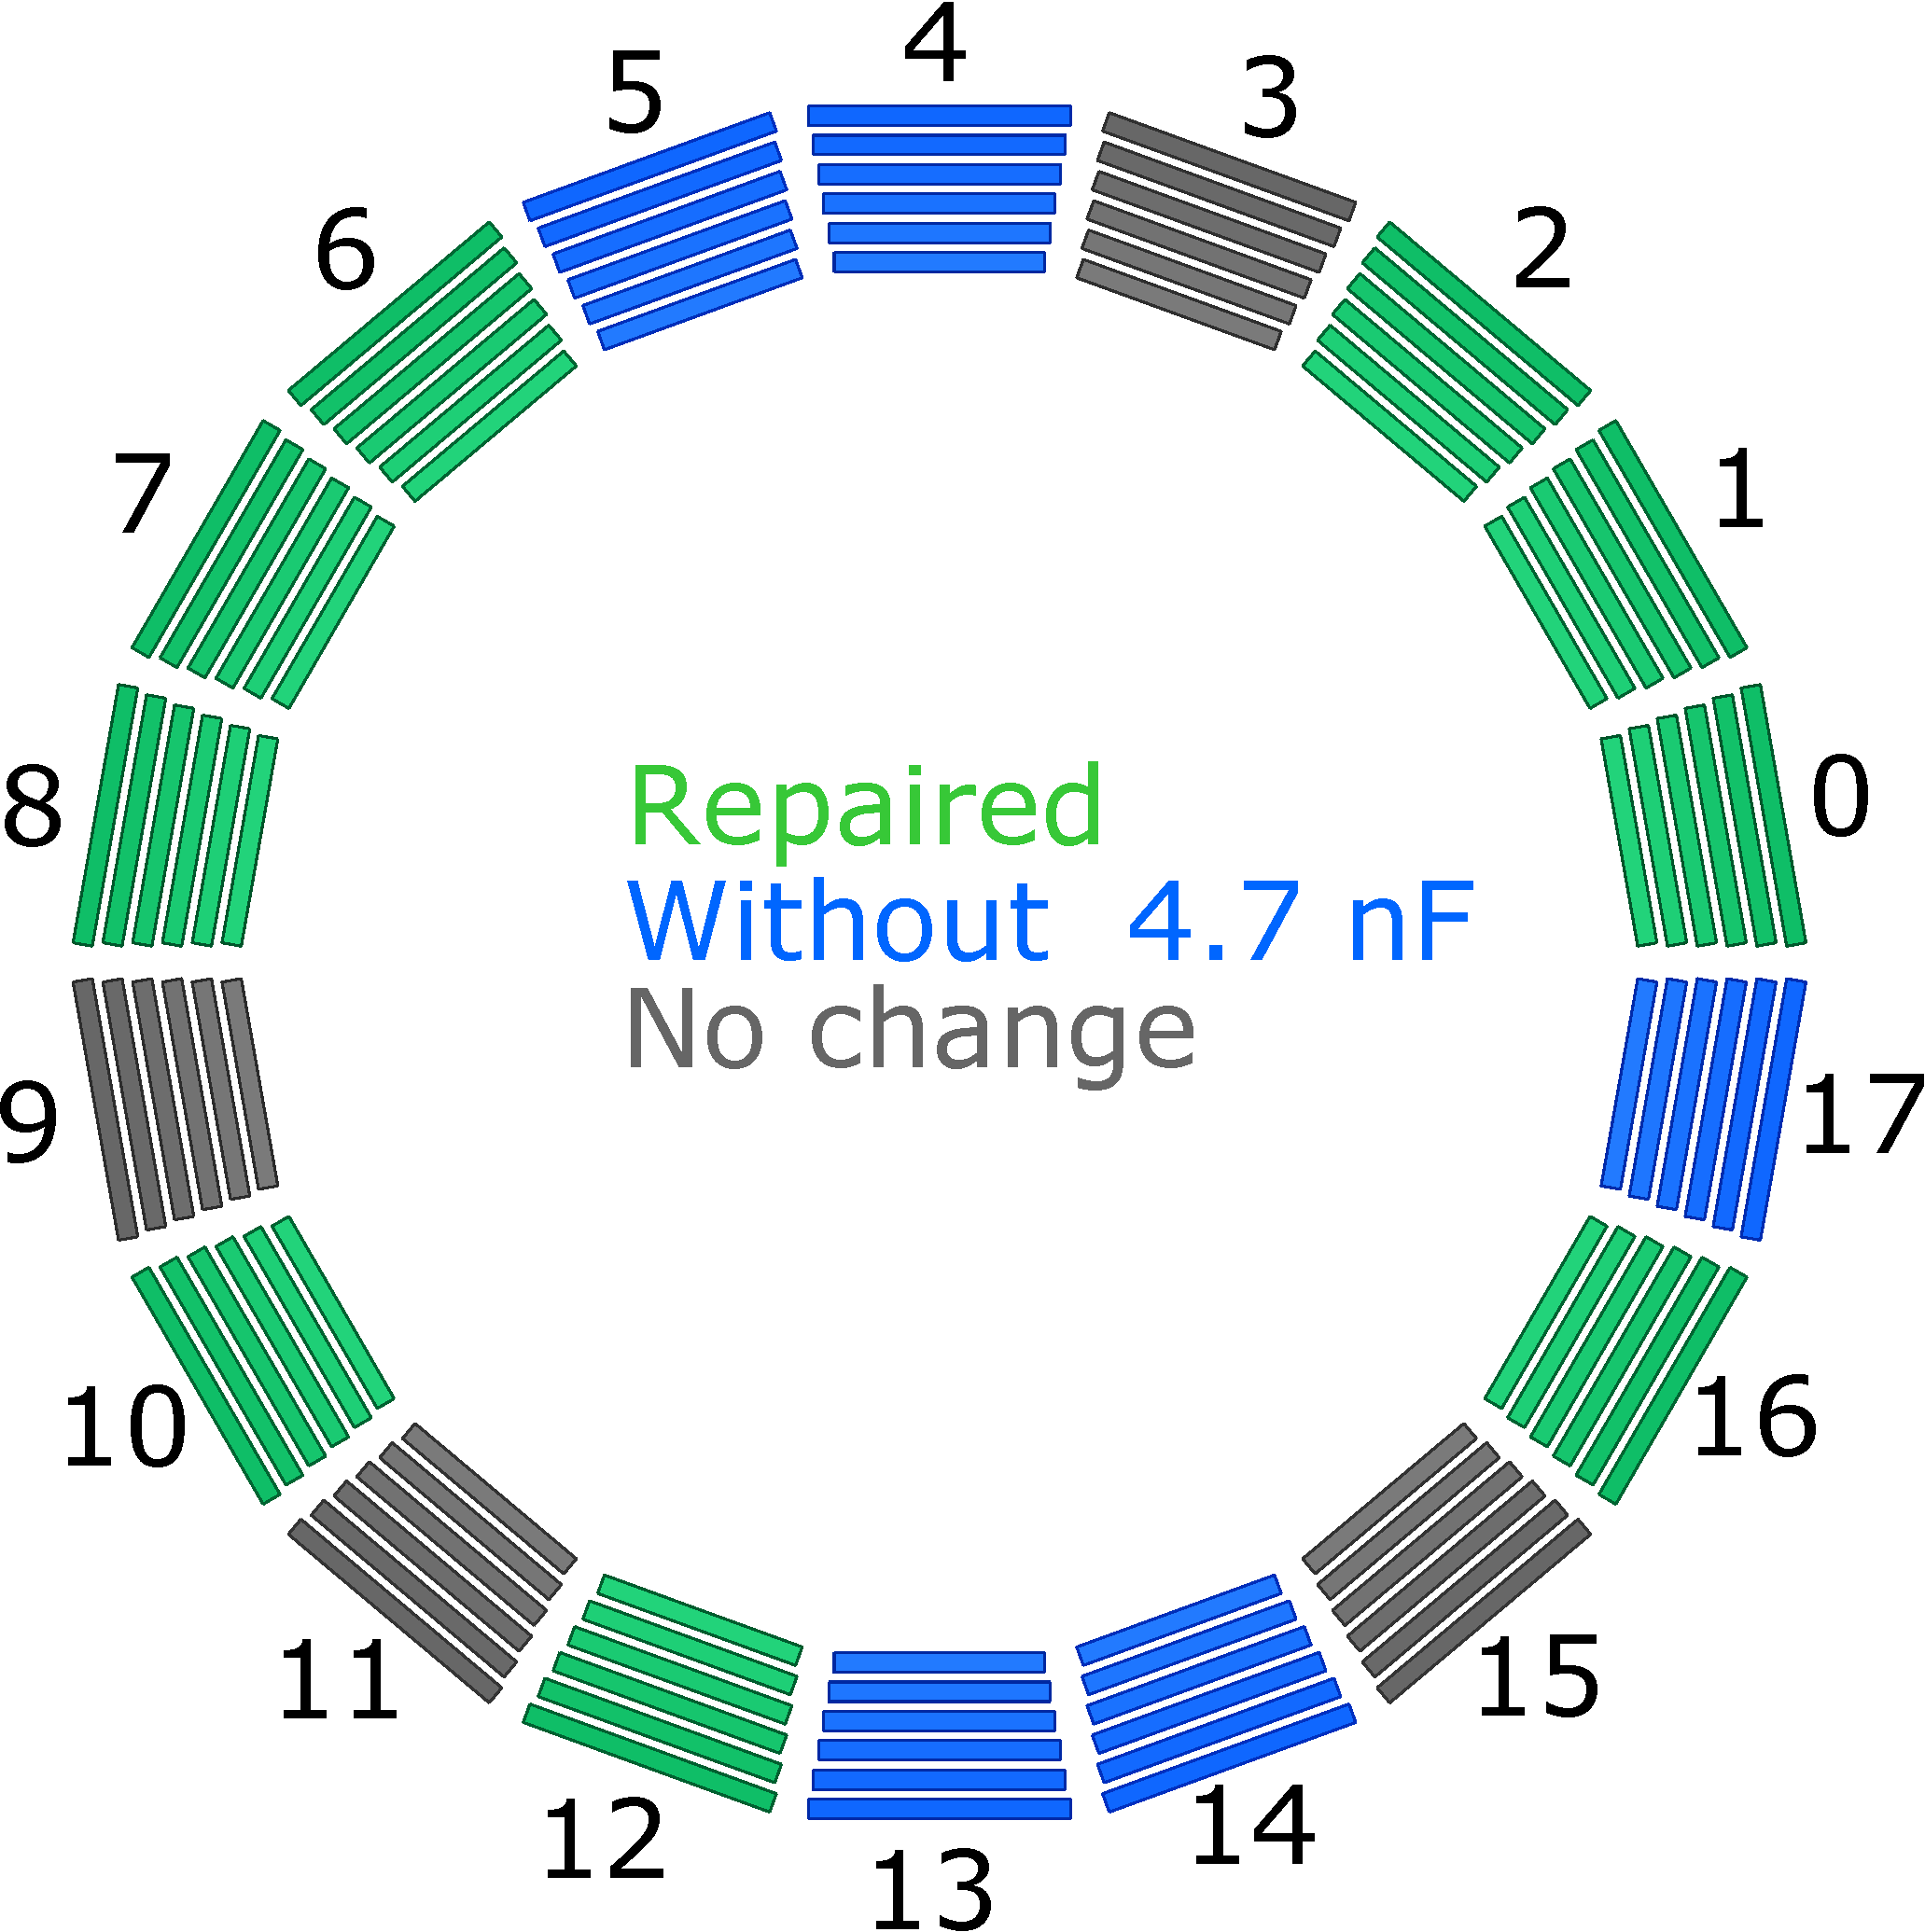
\includegraphics[width=0.5\textwidth]{trd/TRD_front_repaired_label_V2.pdf}
    \caption{The status of SMs concerning capacitors in the HV distribution.}
    \label{fig:TRD_status}
\end{figure}

The HV distribution with the decoupling capacitors on filter boards is mounted directly on each chamber and therefore encased in the hull of the SMs. It was possible to access these locations via milling cut-outs into the casing and removing the top cover to give access to all 30 chambers in a SM. 
Each anode as well as drift channel hold a 4.7 nF capacitor; the anode wire plane is segmented in 8 or 6 sectors of two pad rows each, decoupled from each other by a 2.2 nF capacitor. Measurements of capacitors that were removed confirmed the reason for the HV failures, explaining the observed issues. Most of the problems could be traced to failing 4.7 nF capacitors but it was found that also a small fraction (in the percent range) of the 2.2 nF capacitors had failed. Therefore, all 4.7 nF and 2.2 nF capacitors on the filter boards were removed from a total of 9 TRD SMs. This number was determined by the turn around time of SM deinstallation from the space frame of ALICE, repair, test and reinstallation during the first year of LS2. Before reinstallation of each SM, long-term HV, LV, cooling and readout tests were performed to ensure proper detector operation.
It turned out that 96\% (80 out of 83 not operational chambers) in the 9 SMs could be restored. 
Figure \ref{fig:TRD_status} displays the configuration of the individual SMs in terms of installed decoupling capacitors. Based on experience we estimate that by the end of Run 4 MM chambers in the 4 SMs labelled as unchanged in the figure and NN chambers in the 5 SMs already built without the 4.7 nF capacitors will develop failures. Therefore good tracking capability in all sectors is ensured for the entire planned period of operation. 

As the capacitors were meant to buffer high charge deposits in the chambers, their removal results in larger induced common-mode signals on readout pads in the same high-voltage segment. The measured common-mode signal is shown in Figure \ref{fig:common_mode_ph} and is about three times larger than with the capacitors in place, consistent with the expectation from the remaining capacitance of the readout chamber.
This effect will be corrected in software based on the measured local charge deposit.

\begin{figure}
    \centering
    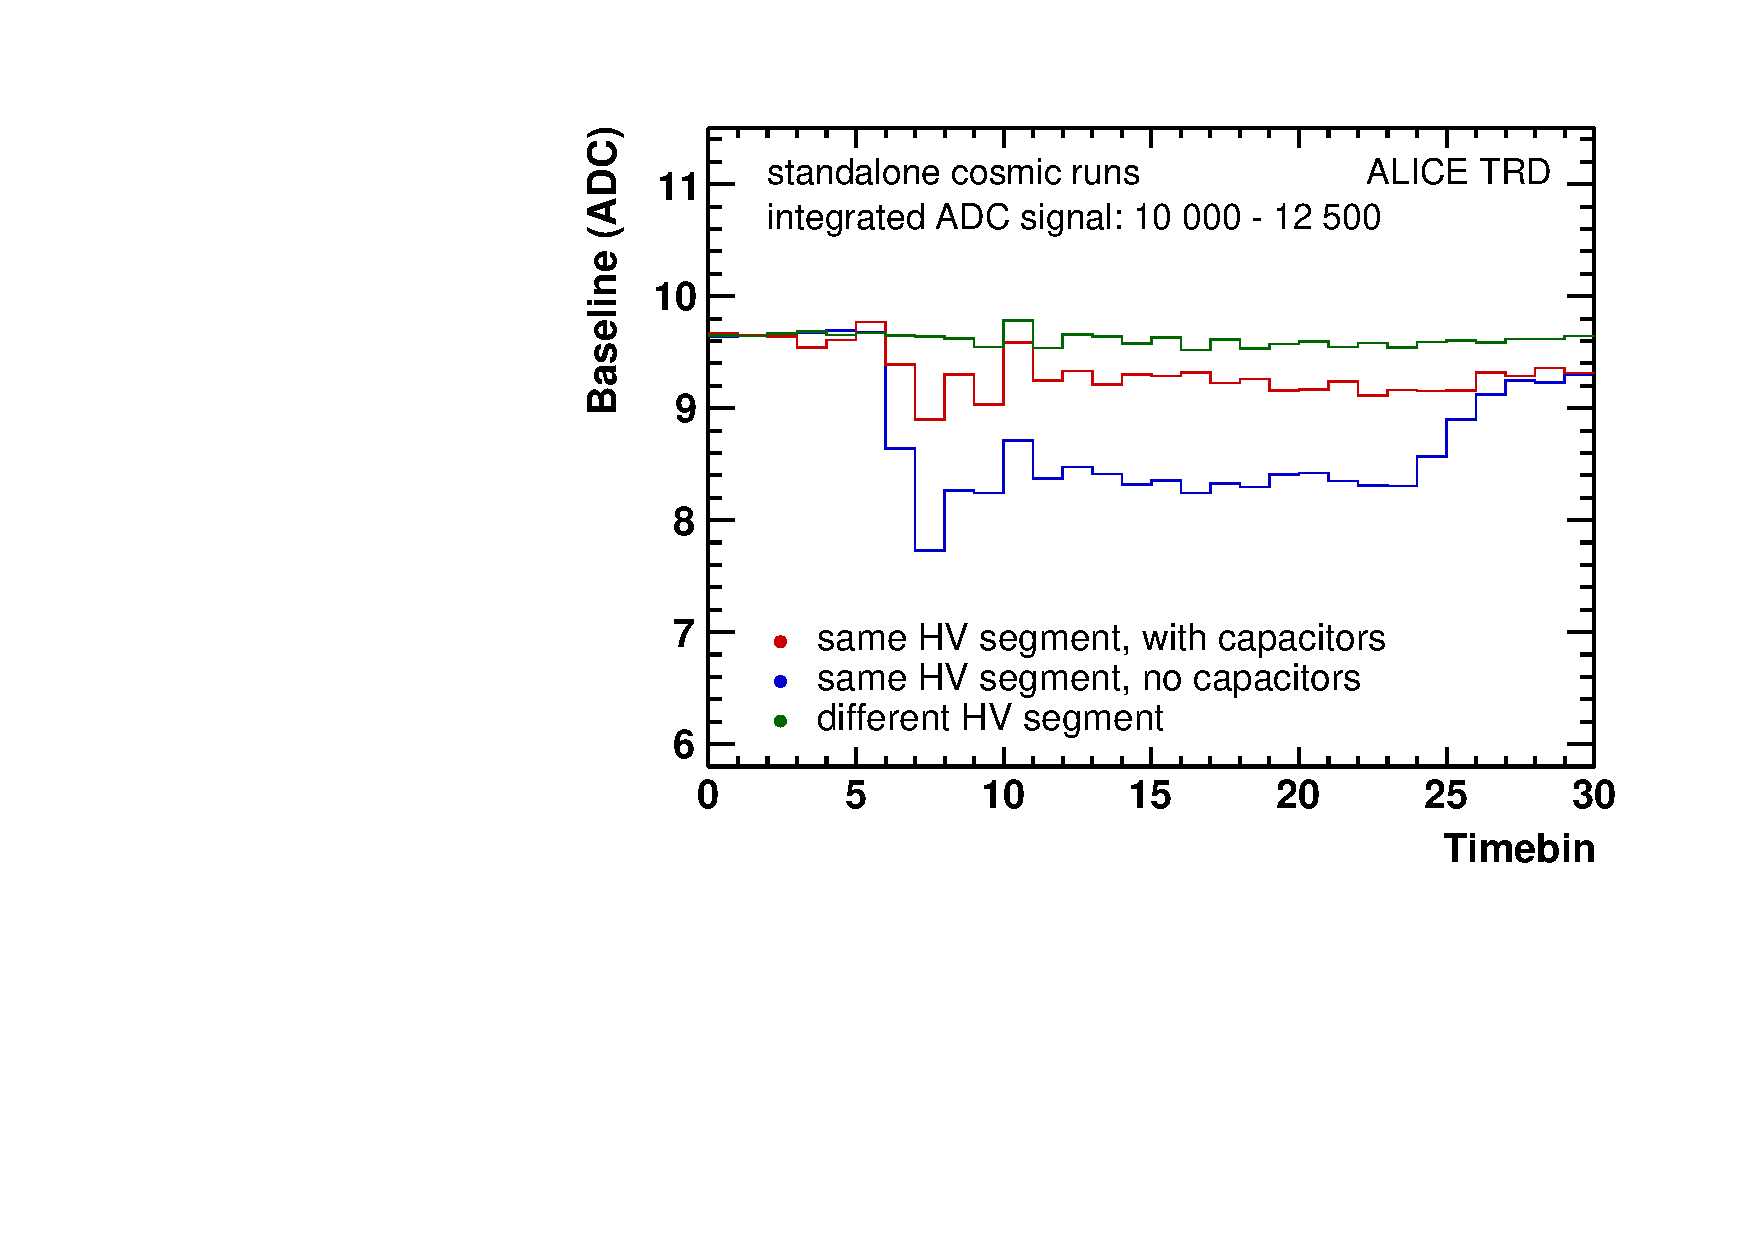
\includegraphics[width=0.6\textwidth]{trd/trd_common_mode.pdf}
    \caption{Induced common-mode signal with and without capacitors for the anode HV. The baseline of pads in the same high-voltage segment as a cosmic ray particle with an integrated signal between 10\,000 and 12\,500 ADC counts is shown before (red) and after (blue) the removal of the capacitors. For comparision, the baseline from pads in high-voltage segment without hits is shown in green.}
    \label{fig:common_mode_ph}
\end{figure}
 
\subsubsection{Readout}

The readout chain has been optimised in the past for a high event inspection rate at LM level with a fast calculation of the L1 trigger contribution (LM tracklet data readout time < \SI{8}{\micro \second} , L1 decision time < \SI{6}{\micro \second}), while transferring large, high resolution raw data for events accepted beyond the L1 level (L1 raw data readout time $\approx$ \SI{300}{\micro \second}). In Run 3, the L1 trigger functionality is no longer required and the detector must provide readout rates as high as feasible while writing all events to permanent storage. No data shall be discarded in the readout chain and the fraction of recorded events in \SI{1}{\mega \hertz} interaction rate pp collisions or \SI{50}{\kilo \hertz} Pb--Pb shall be maximised.

The applied solution is presented in the following sections. Simulations confirm that it enables collecting more than  $\SI{70}{\percent}$ of events in a \SI{50}{\kilo \hertz} interaction rate Pb--Pb running scenario.

\subsubsection{Optimisation of the existing FEE}

In order to achieve a high event readout rate in Run 3, the tracklet readout mode, which has been used to find fast L1 trigger contributions in Run 2, will be used.
The maximum data volume per LM trigger and per Multi Chip Module (MCM) is 4 words of 32 bits each. The usage of the available bits is no longer optimised for triggering, but for physics analysis.

Previously, each MCM processed and transmitted up to 4 tracklets, each as a 32-bit word.
However, even in the most central Pb--Pb events a track density of 4 tracklets per MCM has been rarely reached. Therefore, only 3 tracklets per MCM are allowed in the Run 3 data format. The estimated fraction of tracklets lost by this measure in central Pb--Pb events is below 1\%.
The freed-up 32 bit word is used as a header to store position information about the MCM and 8 bit of PID information per tracklet. It is followed by 1 to 3 32-bit tracklet words that store the position within the MCM, slope and additional 12 bits of PID information of the tracklet. The details are shown in Table \ref{tbl:tracklet:format}.
The PID information per reconstructed tracklet will increase from 8 to 20 bits, which will be used to store charge information from three time slices with 6 or 7 bit dynamic range each. Simulations have shown that the expected performance with this data format is similar to an offline analysis with the same number of time slices. The tracklet position and slope will also be stored with higher precision than in previous runs. 
 
 In previous runs, a preselection cut based on the tracklet inclination has been applied to tracklets in the FEE. This cut is lifted in order to avoid any possibble bias in the collected physics data.
        
In Run 3, the TRD uses a Physics trigger sent by the CTP at LM latency. In addition, the TRD supports a new trigger type, called calibration trigger. The calibration trigger, also sent at LM latency, enables the shipping of Physics data and, additionally, the full raw data. This allows to trigger a full readout for a small fraction of events, facilitating detector calibration. Apart from that, the calibration trigger is interpreted by the FEE as a command to reload its configuration parameters from hamming protected memory areas. This is a precaution measure and mitigates the impact of Single Event Upsets (SEUs) on data taking, sporadically observed on some isolated half chambers as Link Monitor Errors (LMEs) in previous Runs.

\begin{table}[!ht]
    \label{tab:trackletformat}
    \begin{tabular}{lc}
         Header & 
        \bitpattern[startBit=31]
        {1}[1] {padrow}[4] {col}[2] {HPID2}[8] {HPID1}[8] {HPID0}[8] {1}[1]/
         \\
        Payload (1-3x)
        &
        \bitpattern[startBit=31] {position}[11] {LPID}[12] {slope}[8] 0[1]/
    \end{tabular}
  
  \caption[Tracklet data format]{TRD tracklet data format. Each MCM that has reconstructed at least one tracklet will send a header with shared coordinate information and 8 bits of PID information per tracklet. For each reconstructed tracklet, one additional payload word with additional position and PID information as well as the reconstructed tracklet angle (slope) will be stored.}
  \label{tbl:tracklet:format}
\end{table}


\subsubsection{Common Readout Unit (CRU)}

For Run 3, the Global Tracking Unit (GTU) is replaced by CRUs. The CRUs receive the data directly from the FEE via 1080 optical links. Every CRU provides 30 link inputs, implying that in total 36 CRUs are in use. They are housed in 12 First Level Processors (FLPs).

The FPGA firmware on the CRU has been developed in a joint effort between O2 and TRD. It controls the readout process of the detector, receives, buffers and formats the data for the O2 system. All CRUs are connected to the LTU on the CTP side to receive trigger information and to signal a detector busy status to the CTP. Each CRU determines an individual busy status contribution depending on the status of the readout of the connected FEE links. The CTP combines the busy status contributions from all CRUs in order to determine a global busy status of the detector.

The O2 system performs  a deeper level reformatting and data compression before the data is written to permanent storage.
The following points describe sequentially the process of acquiring an event explaining the role of the the CRU and the interactions with other readout components:

\begin{enumerate}
    \item CTP sends a trigger at LM latency (Physics or calibration) via the LTU to the FEE and to the CRUs in parallel. The trigger to the FEE is shipped via the TTC network. The trigger to the CRU is sent via 9 newly set up trigger distribution networks. They use the new Trigger and Timing Control via TTC-PON technology. A large number of networks, 9, is necessary to achieve minimum latency. The CRUs store all information from the received trigger message (e.g. orbit id, bunch crossing id, etc.) in internal buffers.
    
    \item Upon the arrival of the trigger, the FEE begins recording the data while primary charge drifts towards the anode region. Each CRU receives the trigger at approximately the same time and internally opens a time window within which it is waiting for the input links to send all the acquired data. The timeout is programmable. In addition, each CRU generates its busy status contribution and sends it to the CTP. The TTC-PON upstream communication feature is used to transmit the busy status signal. This prevents the CTP from sending any other trigger as long as any CRU contributes an active busy contribution in order to avoid confusion of the FEE state machines.
    
    \item When the FEE has acquired and processed the data, it starts shipping it via TRD custom optical links based on 8b10b encoding. At the end of the transmission, the FEE appends specific end markers. The CRUs record the data received on all input links.
    In case no data end marker is recognised by the CRU within the programmable timeout or data words are received outside the data expectation window, the CRU marks the concerned link as erroneous (LME) and excludes it from data taking until a manual or automated recovery takes place. The CRU stores all received data in large internal data buffers whose size is sufficient to hold even entire calibration data events at maximum measurable multiplicity. When the CRU has confirmed the reception of end makers on all active links or the timeouts have been reached, the CRU releases its busy status contribution. The CTP considers the detector as busy until all 36 CRUs have released their busy contribution. 
    
    \item Once the detector side of the event acquisition is finalised and the data is stored in internal buffers, the CRU is ready to acquire the next event, while at the same time reformatting the buffered data and shipping it to O2. The CRU packs the data into packets of a maximum size of \SI{8}{\kilo B} and equips these packets with Raw Data Headers (RDHs). In addition, TRD-customised headers are inserted into the data stream. The headers contain various information, including the trigger timestamp information, in order to link the acquired data to other detector data during reconstruction.
    
    \end{enumerate}

\subsubsection{DCS}

A special feature of the upgraded TRD DCS system is that the readout chain status of all half chambers is made available to the DCS system by the CRU. The CRU firmware contains a dedicated error state machine for all half chambers. If a connected half chamber shows a misbehavior, which can be detected at the CRU level, the corresponding state machine enters an error state. This error state is stored in a dedicated CRU register, which is read by the DCS system via the ALFRED \cite{Jadlovsky:ICALEPCS2017-THPHA208} architecture. The obtained status of all half chambers is displayed on a dedicated DCS panel in order to monitor LMEs.

\subsubsection{Standalone tracking}
\label{sec:TRD_stand_alone_tracking}
A stand alone tracking algorithm for the TRD was implemented using a Kalman filter approach. The seeding is using the direction and position information of any two TRD tracklets. The track reconstruction efficiency and transverse momentum resolution was determined via matching to tracks from the Time Projection Chamber (TPC).
For the TRD standalone tracking and the current tracklets (without pad tilt correction) a momentum resolution of about 9\% for 500 MeV/$c$ particles was achieved for the case of 6 tracklets in the fit. By including the primary vertex information as an additional constraint, a momentum resolution better than 4\% was achieved. The TRD stand alone tracking algorithm was so far already used to identify and study photon conversions and nuclear interactions in front of and within the TRD. It will also be used for the TRD drift velocity calibration in Run 3.

\subsubsection{Calibration}

The Run 3 TRD calibration procedure is similar to the one employed before, except for the drift velocity calibration, which will be based on a new development. The angle between a TRD tracklet and the corresponding TRD standalone track, $\Delta \alpha$, is measured as a function of the track impact angle for each chamber. 
A model which includes as free parameters the effective drift velocity $v_{D}^{eff}$ and the Lorentz angle $\alpha_{L}$ is used to fit the distributions. An example for detector 7 is depicted in Fig. \ref{fig:calibrate_5} (left). The effective drift velocity is compensating the ion tail effect which is systematically changing the tracklet angle. The physical true drift velocity $v^{true}_{D}$ is about 35\% larger than $v_{D}^{eff}$. A closure test with 50k events was performed using Run 2 data and the new $v_{D}^{eff}$ parameters. The average angular difference between tracklets and TRD track is zero, as shown in Fig. \ref{fig:calibrate_5} (right).

\begin{figure}[htb]
  \centering
    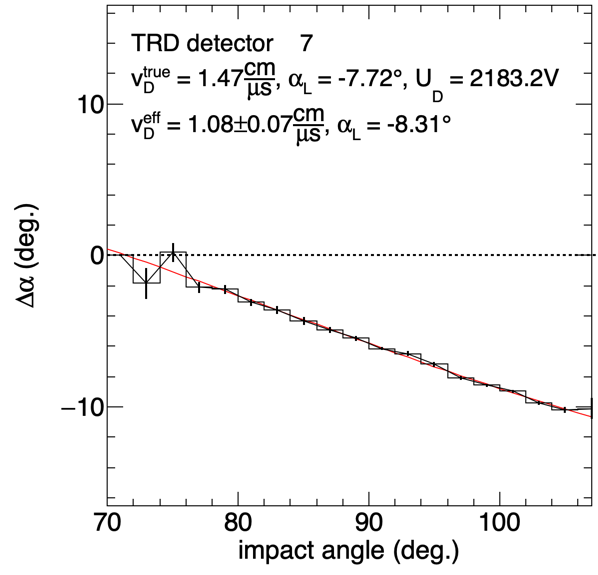
\includegraphics[width=0.42\linewidth]{Delta_alpha_vs_impact_angle.png}
    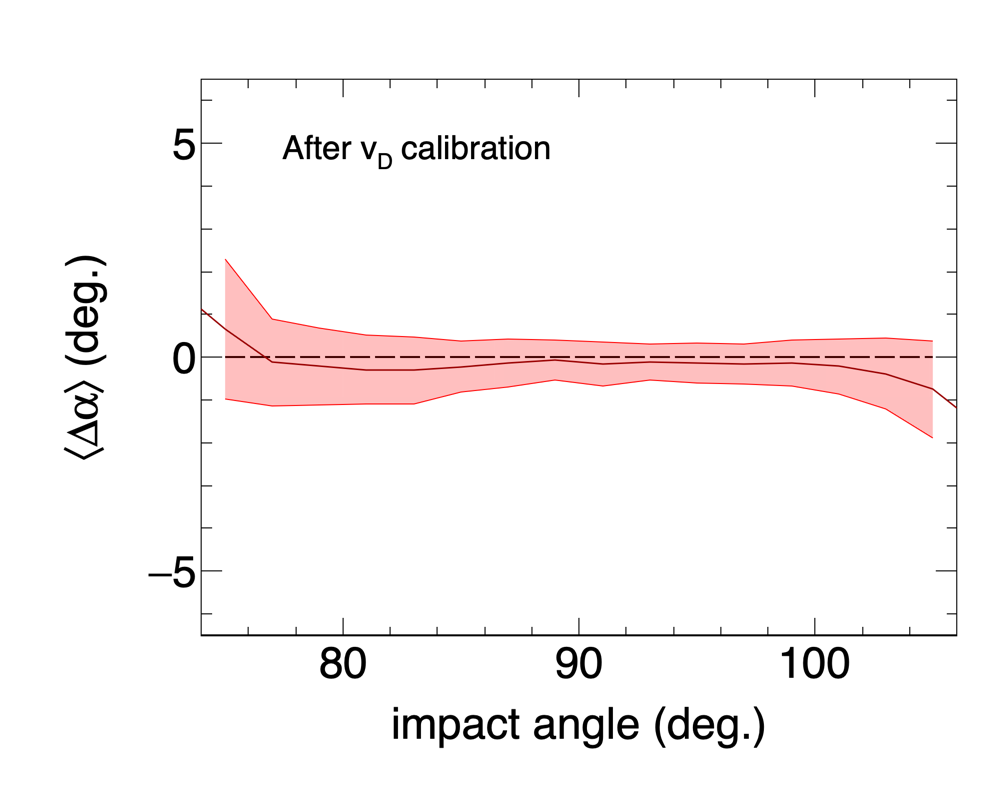
\includegraphics[width=0.45\linewidth]{Delta_alpha_after_calib_V4.png}
  \caption{Left: $\Delta\alpha$ versus impact angle for a typical TRD chamber in Run 2, having a fixed uncalibrated drift velocity. The upper values refer to the Run 2 calibration procedure, the lower ones to the new calibration scheme. Right: Average $\Delta\alpha$ versus impact angle distribution for all TRD detectors after the calibration was applied. The red band shows the RMS of the distribution.}
  \label{fig:calibrate_5}
  \end{figure}

About 100k MB p--Pb equivalent events are needed for an update of the calibration parameters. This is similar to what was used in the past in Run 2 with about 600-3000 good tracklets per chamber. The seeding and Kalman filter procedures need on average 10 ms per p--Pb event. In total, not more than 20 minutes for one update of the calibration parameters is needed on a single CPU core. 
The time consuming tracking part will be parallelized.

\subsubsection{Quality Control}

The O2 system for the TRD will use the Quality Control (QC) framework to consolidate the online Data Quality Monitoring (DQM) and offline Quality Assurance (QA) into a single system. The QC system consists of tasks that are running in various parts of the O2 system and produce QC objects, mostly in the form of histograms.

\begin{itemize}

    \item Raw data format. The data arriving from the FEE via the CRU is validated, allowing to detect disabled or malfunctioning parts in the readout tree or SEUs in the FEE. 
    
    \item Zero-suppressed ADC data from all calibration events will be analyzed to reconstruct the average, time-dependent signal shape for each of the 522 readout chambers. These histograms are a versatile low-level monitoring tool for many aspects of the operation of the TRD, including trigger timing, drift velocity and gas gain.
    
    \item Tracklets from a small fraction of events complement the ADC data QC and monitor the local reconstruction of track segments in the FEE of each chamber.
    
    \item Tracking QC will run during synchronous and asynchronous reconstruction and monitor the efficiency at the tracklet and track level.
    
    \item Residuals between reconstructed tracks and tracklets are analyzed in the asynchronous stage to monitor the impact of alignment and calibration on the detector performance.
\end{itemize}

The data from these QC tasks is further processed by checker algorithms to provide automated notifications and trending. 

